\documentclass[en]{../../../eplsummary}

\usepackage{listings}


\lstset{
  frame=top,frame=bottom,
  basicstyle=\small\normalfont\sffamily,    % the size of the fonts that are used for the code
  stepnumber=1,                           % the step between two line-numbers. If it is 1 each line will be numbered
  numbersep=10pt,                         % how far the line-numbers are from the code
  tabsize=2,                              % tab size in blank spaces
  extendedchars=true,                     %
  breaklines=true,                        % sets automatic line breaking
  captionpos=t,                           % sets the caption-position to top
  mathescape=true,
  stringstyle=\color{white}\ttfamily, % Farbe der String
  showspaces=false,           % Leerzeichen anzeigen ?
  showtabs=false,             % Tabs anzeigen ?
  xleftmargin=17pt,
  framexleftmargin=17pt,
  framexrightmargin=17pt,
  framexbottommargin=5pt,
  framextopmargin=5pt,
  showstringspaces=false      % Leerzeichen in Strings anzeigen ?
 }

\DeclareCaptionFormat{listing}{\rule{\dimexpr\textwidth+17pt\relax}{0.4pt}\par\vskip1pt#1#2#3}
\captionsetup[lstlisting]{format=listing,singlelinecheck=false, margin=0pt, font={sf},labelsep=space,labelfont=bf}

\renewcommand\lstlistingname{Algorithm}

\tikzset{
r/.style = {treenode, circle, text width=1.5em, very thick}
}

\DeclareMathOperator{\scp}{scp}
\DeclareMathOperator{\rel}{rel}
\DeclareMathOperator{\sol}{sol}

\hypertitle{Constraint Programming}{8}{INGI}{2365}
{Houtain Nicolas}
{Yves Deville}

\section{Constraint Programming (CP)}
\textsc{CP = Model + Search}

\begin{enumerate}
    \item \textsc{Model} : Describe real world problem with
        \begin{itemize}
            \item \textbf{Variables} : $X = \{x_1, x_2,\cdots, x_n\}$
            \item \textbf{Domains} : $D = \{ D(x_1), D(x_2),\cdots,
                D(x_n)\}$

                \begin{itemize}
                    \item[Ex:] Booleans, \textbf{finite domains}, finite
                        set, intervals, continuous domains,\ldots
                \end{itemize}
            \item \textbf{Constraints} : $C = \{c_1, c_2,\cdots, c_e\}$
                \begin{itemize}
                    \item A \textbf{scope} $\scp(c) = (x_1, x_2,\cdots,x_r)$ : is the
                        variables constrained by c.
                    \item A \textbf{relation} $\rel(c)$ : value combinations accepted by
                        c
                \end{itemize}
            \item \textbf{Objective function} : $O : \sol \to \R$
        \end{itemize}

        \paragraph{Types}
        \begin{enumerate}
            \item CSP${} = (X, D, C)$
            \item COP${} = (X, D, C, O)$
        \end{enumerate}

        \paragraph{Declarative} : describe what you want not how to get it
    \item[+]
    \item \textsc{Search} : Describe how to solve the problem.
        \begin{itemize}
            \item \textbf{Propagation} : Use constraints to remove
                \textit{useless} (doesn't remove solution) parts of the search space
                \begin{center}
                    \scriptsize
                    \textit{Need choice between more pruning with more
                        expensive to compute or less proning cheaper to
                    compute}
                \end{center}

                \begin{itemize}
                    \item Consistencies : Require that all the values
                        are able to satisfy their constaints in
                        \textbf{isolation}

                    \item Propagator: used at the beginning of the search
                        and each time a decision is made.
                \end{itemize}
            \item \textbf{Backtracking Tree Search} : Explore search
                space by taking decisions and backtracking (with
                remembering decision)

                \paragraph{Current node}: The node is modified at each decision
                made and it is restored when backtracking occurs.
        \end{itemize}

        \paragraph{Search space} = $D(x_1) \times D(x_2) \times \cdots \times D(x_n)$
\end{enumerate}


\paragraph{Solution}
A solution to a CSP is
\begin{enumerate}
    \item An assigment of variables at values in their domains
    \item Such that all the constraints are respected
\end{enumerate}

% TODO ---v %
\subsection{Auxiliary variables}
\begin{center}
  \begin{tabular}{c}
    Variables used to help/improve modeling\\
    VS\\
    Variables which represent the decision CP has to make
  \end{tabular}
\end{center}

\paragraph{redundant constraint} constraint that does not exclude any previous solution,
improve pruning (reduce search space), improve communication

\subsection{Global constraint}

\subsection{Symmetry}





\section{Propagation}
\begin{itemize}
    \item $n$ variables
    \item domains of size $d$
    \item $e$ constraints
    \item maximum arity $r$
\end{itemize}

\begin{table}
    \centering
\begin{tabular}{|c|c|c|c|c|}
    \hline
    & Algo & Complexity & Type & Other \\
    \hline
    \hline
    \multirow{3}{*}{\rotatebox{90}{\scriptsize Constraint}}
    & GAC3 & $\bigoh(e \times r^3 \times d^{r+1})$ & $n$-ary & \\
    & AC3rm & $\bigoh(e \times d^3)$ & binary & Residues \& multidirectionality\\
    & AC2001 & $\bigoh(e \times d^2)$ & binary &  firstSupport(x, a)\\

    \hline
    \hline
    \multirow{2}{*}{\rotatebox{90}{\scriptsize Value}}
    & GAC4 & $\bigoh(e \times r \times d^r)$ & $n$-ary & c.support(x,a) \\
    & AC6 & $\bigoh(e \times d^2)$ & binary & firstSupported(x, a) \\
    \hline
\end{tabular}
\caption{Generic propagator algorithm}
\end{table}

\begin{table}
    \centering
    \begin{tabular}{|m{5cm}|m{5cm}|m{5cm}|}
        \hline
        CB & Collect and propagate & VB \\
        \hline

        c in Q & c in Q & (c, x, a) in Q \\

        \begin{itemize}
            \item called once for each set of change in SP
            \item re-enforce the whole consistency
            \item no information on changes
        \end{itemize}
        &
        &
        \begin{itemize}
            \item called once for each single change in SP
            \item reflects only one change at a time ($a \notin D(c)$)
            \item information on each change, one at a time
        \end{itemize}
        \\

        \hline

        \small
        \begin{enumerate}
            \item \textcolor{red}{less} information
            \item called \textcolor{green}{less}
        \end{enumerate}
        
        &
        \small
        \begin{enumerate}
            \item \textcolor{green}{more} information
            \item called \textcolor{green}{less}
        \end{enumerate}
        
        &
        \small
        \begin{enumerate}
            \item \textcolor{green}{more} information
            \item called \textcolor{red}{more}
        \end{enumerate}
        
        \\

        \multicolumn{3}{c}{\begin{tikzpicture}
            \draw[<->] (0,0) -- (13, 0);
        \end{tikzpicture}}\\

    \end{tabular}
    \caption{Fixed point}
\end{table}

\subsection{Without propagation (Bruteforce)}

\begin{tabular}{m{6cm}cm{6cm}}
    \begin{itemize}
        \item $\bigoh(d^n)$ possible assignements
        \item $\bigoh(r)$ to test a constraint
        \item $\bigoh(e \times r)$ to test all constraint
    \end{itemize}
    & $\to$ &
    \textbf{Global complexity}: $\bigoh(d^n \times e \times r)$
\end{tabular}

\subsection{Fonctionnement}

The goal of propagation is to \textbf{reduce} the search space
(\textit{reduction domains, reduction constraints, addition constraint})
but do not remove solutions.

The propagation is used before the search and all along the search.

\subsubsection{Partial solution}

A partial instantiation gives values to some variables.
It's a \textbf{partial solution} IFF
\begin{center}
    for all constraint c : if all variables assigned $\to$ c satisfied
\end{center}


The propagation perfom checking and \textcolor{red}{fail} when there is
no partial solution : checking fails or there is inconsistency (empty domain,\ldots)

\subsubsection{Level of propagation}
\begin{center}
\begin{tabular}{ccc}
    \textbf{Weaker} & $\Leftrightarrow$ & \textbf{Stronger} \\
    Less pruning & & More pruning \\
    Cheaper to compute & & More expensive to compute \\
\end{tabular}
\end{center}


\subsection{Constraint based propagation}

\subsubsection{Fixed point algorithm}

The propagator must implements two methods :
\begin{enumerate}
    \item \texttt{setup()} : initialize the constraint
    \item \texttt{propagate()} : compute the set of values that are inconsistent

    \item[$\to$] \texttt{removeValue(a, D(x))} fails if D(x) empty
\end{enumerate}

\paragraph{Note:} use GAC consistency

\begin{lstlisting}[mathescape, caption=CB Fixed point]
initCBDomFilter(Q){
    for(c $\leftarrow$ C){
        c.setup()
        Q += c
    }
}

CBDomFilter(X, D, C){
    Q = $\emptyset$
    initCBDomFilter(Q)
    propagateQueueCBDomFilter(Q)
}

propagateQueueCBDomFilter(Q){
    while(Q $\neq$ $\emptyset$){
        c = popCtrt(Q)
        $\Delta$ = c.propagate()
        for((x,a) $\leftarrow$ $\Delta$){
            removeValue(a,D(x))
            for(c $\leftarrow$ C/{c} if c.scope contains x){
                if(! Q contains c)
                    Q += c
            }
        }
    }
}

\end{lstlisting}

\subsubsection{Generic GAC}

The only requirement is a test method for the constraint which say \textit{true/false}
if the given value is right.


\begin{enumerate}
    \item \textbf{GAC3} \begin{lstlisting}[mathescape, caption=GAC3]
setup(){}

propagate(){
    $\Delta$ = $\emptyset$
    for(x $\leftarrow$ scope){
        for(a $\leftarrow$ D(x)){
            if( $\forall$(v $\leftarrow D(scope)_{x=a})$ (! c(v)) )
                // No combination with x=a satisfying the constraint
                $\Delta$ += (x, a)
        }
    }
    return $\Delta$
}
    \end{lstlisting}

    \begin{tabular}{m{7cm}cm{6cm}}
        \begin{itemize}
            \item $\bigoh(r^2 \times d^r)$ for \texttt{propagate()}
            \item $\bigoh(r \times d)$ calls of \texttt{propagate()} in \texttt{propagateQueueCBDomFilter()}
        \end{itemize}
        & $\to$ &
        \textbf{Global complexity}: $\bigoh(e \times r^3 \times d^{r+1})$
    \end{tabular}

\item \textbf{AC3rm} : the idea is to add memory by check the last found
    support first.
    \paragraph{AC3 with }
    \begin{itemize}
        \item Residues :  \texttt{c.support(x, a)} = last found support for (x, a)

        \item Multidirectionality : if $b$ is a support for $a$, then $a$ is
            a support for $b$
    \end{itemize}

\paragraph{Note: } Propagator for binary constraints ($\scp(c)=(x, y)$)

\begin{lstlisting}[mathescape, caption=AC3rm]
setup(){
    for(a $\leftarrow D(x)$) { support(x, a) = $\bot$}
    for(b $\leftarrow D(y)$) { support(y, b) = $\bot$}
}

propagate(){
    $\Delta_1$ = propagate_var(x)
    $\Delta_2$ = propagate_var(y)
    return $\Delta_1 \cup \Delta_2$
}

propagate_var(x){
    $\Delta$ = $\emptyset$
                            // Residues
    for(a $\leftarrow$ D(x) if (! D(y) contains support(x, a))){
        b = y.min
        while(b != $\top$ && ! c(x=a, y=b)){
            b = y.valueAfter(b)
        }
        if( b == $\top$ )
            $\Delta$ += (x, a)
        else {
            // Multidirectionality
            support(x, a) = b
            support(y, b) = a
        }
    }

    return $\Delta$
}
    \end{lstlisting}

    \begin{tabular}{m{7cm}cm{6cm}}
        \begin{itemize}
            \item $\bigoh(d)$ for \texttt{setup()}
            \item $\bigoh(d^2)$ for \texttt{propagate()}
            \item $\bigoh(d)$ calls of \texttt{propagate()} in \texttt{propagateQueueCBDomFilter()}
        \end{itemize}
        & $\to$ &
        \textbf{Global complexity}: $\bigoh(e \times d^3)$
    \end{tabular}

    \paragraph{Backtrack}: when we backtrack, AC3rm only search support for
    values that have lost theirs. When needed, the backtracking scan \textbf{all
    the domain} of the other variable!

    $\to$ AC2001 to optimise the backtracking

\item \textbf{AC2001} : to avoid to scan \textit{all the domain}, a node
keep the firstSupport which may be restore when backtracking.

\paragraph{Note: } Propagator for binary constraints ($\scp(c)=(x, y)$)

\begin{lstlisting}[mathescape, caption=AC2001]
setup(){
    for(a $\leftarrow D(x)$) { support(x, a) = $\bot$}
    for(b $\leftarrow D(y)$) { support(y, b) = $\bot$}

propagate(){
    $\Delta_1$ = propagate_var(x)
    $\Delta_2$ = propagate_var(y)
    return $\Delta_1 \cup \Delta_2$
}

propagate_var(x){
    $\Delta$ = $\emptyset$
                            // Residues
    for(a $\leftarrow$ D(x) if (! D(y) contains support(x, a))){
        b = y.valueAfter(firstSupport(x,a))
        while(b != $\top$ && ! c(x=a, y=b)){
            b = y.valueAfter(b)
        }
        firstSupport(x, a) = b

        if( b == $\top$ )
            $\Delta$ += (x, a)
    }

    return $\Delta$
}
\end{lstlisting}

\begin{tabular}{m{7cm}cm{6cm}}
    \begin{itemize}
        \item $\bigoh(d)$ for setup()
        \item $\bigoh(d)$ for one literal, all updates of firstSupport
        \item $\bigoh(d)$ for one literal, validity of firstSupport checked
        \item $\bigoh(d^2)$ for propagate()
    \end{itemize}
    & $\to$ &
    \textbf{Global complexity}: $\bigoh(e \times d^2)$
\end{tabular}

\end{enumerate}

\subsubsection{Specific}
We can improme the previous complexity if we have a propagator specific
for a constraint.

\begin{lstlisting}[caption=Specific propagator for x <= y + k, mathescape]
propagate(){
    $\Delta$ = $\emptyset$
    a = x.max
    while(a != $\bot$ && a > y.max + k){
        $\Delta$ += (x, a)
        a = x.valueBefore(a)
    }

    b = x.min
    while(b != $\bot$ && b < x.min - k){
        $\Delta$ += (y, b)
        b = x.valueAfter(b)
    }

    return $\Delta$
}
\end{lstlisting}


\subsection{Value based propagation}

In this case, the queue contains constraints and literals $(c,x,a)$.
c has to reflect that $a \notin$ D(x).

\begin{itemize}
    \item[+] efficient filtering
    \item[-] called for each literal removed
\end{itemize}


\paragraph{Treat inconsistent values because $a \notin D(x)$}
c considers (c, y, b) on Q are sill in the domains!

\begin{itemize}
    \item $\gamma$ on X is \textbf{valid} iff $\forall$ x $\in$ X : $\gamma(x) \in D(x)$
    \item $\gamma$ on X is \textbf{Q-valid} iff $\forall$ x $\in$ X : $\gamma(x) \in D(x)
        \cup \{a | (c, x, a) \in Q\}$
\end{itemize}


\subsubsection{Fixed point algorithm}
In this case, the propagator must implement :
\begin{enumerate}
    \item \texttt{setup()} : initialize the constraint
    \item \texttt{valRemove(x, a)} : computes the set of values that are
        inconsistent because $a \notin D(x)$
\end{enumerate}

\paragraph{Note:} use GAC consistency

\begin{lstlisting}[mathescape, caption=CB Fixed point]

initVBDomFilter(X, D, C){
    Q = $\emptyset$
    C1 = $\emptyset$
    for(c $\leftarrow$ C){
        $\Delta$ = c.setup()
        for( (x, a) $\leftarrow$ $\Delta$){
            removeValue(a, D(x))
            for( c $\leftarrow$ C1 if c.scope contains x){
                if(! Q contains (c, x, a))
                    Q += (c, x, a)
            }
        }
        C1 += c
    }
}

VBDomFilter(X, D, C){
    Q = $\emptyset$
    initVBDomFilter(Q)
    propagateQueueVBDomFilter(Q)
}

propagateQueueVBDomFilter(Q){
    while(Q $\neq$ $\emptyset$){
        (c, x, a) = popCtrtLiteral(Q)
        $\Delta$ = c.valRemove(x, a)
        for((x,a) $\leftarrow$ $\Delta$){
            removeValue(a,D(x))             
            for(c $\leftarrow$ C/{c} if c.scope contains x){
                if(! Q contains (c, x, a))
                    Q += (c, x, a)
            }
        }
    }
}

\end{lstlisting}


\subsubsection{Generic}

\begin{enumerate}
    \item \textbf{GAC4} maintains sets of supports for literals (x,a) :
        \begin{center}
            c.support(x,a) = \{ $\gamma \in D(c.scope, Q, c)_{x=a} : c(\gamma)$\}
        \end{center}

        In this way, we removes Q-invalid support and when no more supports,
        ce can removed them to D(x).

        \paragraph{Note:} c.support must be backtracked during search

\begin{lstlisting}[mathescape, caption=GAC4]
setup(){
    $\Delta$ = $\emptyset$

    // Initialisation of support data structure
    for(x $\leftarrow$ scope){
        for( a $\leftarrow$ D(x))
            support(x, a) = $\emptyset$
    }
    for($\gamma \leftarrow$ scope if c($\gamma$)){
        for( x $\leftarrow$ scope)
            support(x, $\gamma(x)$) += $\gamma$
    }

    // First pruning
    for( x $\leftarrow$ scope){
        for( a $\leftarrow$ D(x)){
            if(support(x, a) == $\emptyset$)
                $\Delta$ += (x, a)
        }
    }

    return $\Delta$
}

valRemove(x, a){
    $\Delta$ = $\emptyset$
    for( $\gamma \leftarrow$ support(x, a)) {
        for(y $\leftarrow$ scope if y $\neq$ x if D(y) contains b){

            // $\gamma$ is a support for (y, $\gamma(y)$) and $\gamma$ is Q-invalid
            b = $\gamma(y)$
            support(y, b) -= $\gamma$
            if( support(y, b) == $\emptyset$)
            $\Delta$ += (y, b)
        }
    }

    return $\Delta$
}
\end{lstlisting}

    \begin{tabular}{m{7cm}cm{6cm}}
        \begin{itemize}
            \item $\bigoh(r \times d^r)$ for \texttt{setup()}
            \item $\bigoh(r \times d^r)$ for all calls to \texttt{valRemove()}
                because \textbf{each support} is considered \textbf{once}
        \end{itemize}
        & $\to$ &
        \textbf{Global complexity}: $\bigoh(e \times r \times d^r)$
    \end{tabular}


\item \textbf{AC6}: similar to AC2001 because use structure \texttt{firstSupported}

    \paragraph{firstSupported(x,a)}
    \begin{itemize}
        \item (x,a) is the first support of (y,b) ($b \in $firstSupported(x,a))
        \item[$\to$] when (x,a) removed, AC6 know which values in D(y) need a new first support
    \end{itemize}

\begin{lstlisting}[mathescape, caption=AC6]
setup(){
    $\Delta = \emptyset$
    $\Delta += $ setup_var(x)
    $\Delta += $ setup_var(y)
}

setup_var(x){
    $\Delta$ = $\emptyset$
    for( b $\leftarrow$ D(y))
        firstSupported(y, b) = $\emptyset$

    for( a $\leftarrow$ D(x)) {
        b = y.min
        while( b != $\top$ && !c(x=a, y=b)){
            b = y.valueAfter(b)
        }

        if(b == $\top$)
            $\Delta$ += (x, a)
        else
            firstSupported(y, b) += a
    }

    return $\Delta$
}

valRemove(x, a){
    $\Delta$ = $\emptyset$

    // All value that need new support
    for(b $\leftarrow$ firstSupported(x,a) if D(y) contains b){
        a' = x.valueAfter(a)
        while(a' != $\top$ && !c(x=a, y=b))
            a' = x.valueAfter(a')

        if(a' == $\top$)
            $\Delta$ += (y, b)
        else
            firstSupported(x, a') += b
    }
    return $\Delta$
}
\end{lstlisting}

    \begin{tabular}{m{7cm}cm{6cm}}
        \begin{itemize}
            \item $\bigoh(d^2)$ for \texttt{setup()}
            \item $\bigoh(d)$ for one literal, all searches for support
            \item $\bigoh(d^2)$ for all calls to \texttt{valRemove()}
        \end{itemize}
        & $\to$ &
        \textbf{Global complexity}: $\bigoh(e \times d^2)$
    \end{tabular}

\end{enumerate}

\subsubsection{Specific}

\subsection{Collect and propagate}

It's a mixing constraint and value based. When the propagor is called it
know all the change at one with \texttt{propagate($\Delta_c$)}

\begin{itemize}
    \item A propagation queue of constraints
    \item a $\Delta_c$ (= all literal removed since last call to c) fore each constraints
\end{itemize}

\subsubsection{Fixed point algorithm}
In this case, the propagator must implement :
\begin{enumerate}
    \item \texttt{setup()} : initialize the constraint and performs first pruning
    \item \texttt{propagate($\Delta_c$)} : compute the set of values that are inconsistent because
        $\Delta_c \notin D$
\end{enumerate}

\paragraph{Note:} use GAC consistency

\begin{lstlisting}[mathescape, caption=CB Fixed point]

initCPDomFilter(X, D, C){
    Q = $\emptyset$
    C1 = $\emptyset$
    for(c $\leftarrow$ C){
        $\Delta$ = c.setup()
        for( (x, a) $\leftarrow$ $\Delta$){
            removeValue(a, D(x))
            for( c $\leftarrow$ C1 if c.scope contains x){
                if(! Q contains c)
                    Q += c
                $\Delta_c$ += (x, a)
            }
        }
        C1 += c
    }
}

CPDomFilter(X, D, C){
    Q = $\emptyset$
    initCPDomFilter(Q)
    propagateQueueCPDomFilter(Q)
}

propagateQueueCPDomFilter(Q){
    while(Q $\neq$ $\emptyset$){
        (c) = popCtrt(Q)
        $\Delta$ = c.propagate($\Delta_c$)
        $\Delta_c$ = $\emptyset$
        for((x,a) $leftarrow$ $\Delta$){
            removeValue(a,D(x))
            for(c $\leftarrow$ C/{c} if c.scope contains x){
                if(! Q contains c)
                    Q += c
                $\Delta_c$ += (x,a)
            }
        }
    }
}

\end{lstlisting}






\section{Consistency}

\paragraph{CSP} A CSP (\textsc{X, D, C}) is $X_{Consistent}$ iff all
constraints $c \in C$ are $X_{Consistent}$,

where $X_{Consistent}$ is GAC, BC,\ldots



\paragraph{Propagation strength}
A consistency $S_1$ is stronger than a consistency $S_2$ iff all CSP respecting
$S_1$ also respect $S_2$.

(Some consistencies can be \textit{incomparable})

\begin{table}[!h]
    \centering
    \begin{tabular}{l|c|c|}
        \cline{2-3}
        \multirow{3}{*}{\begin{tikzpicture}
            \draw[->] (0,0) edge node [left]{\rotatebox{90}{Strongest}} (0, 1.5);
        \end{tikzpicture}} &
        Singleton GAC & maxRPWC \\
        \cline{2-3}
        & \multicolumn{2}{c|}{GAC} \\
        \cline{2-3}
        & Bound consistency & Forward checking \\
        \cline{2-3}
    \end{tabular}
    \caption{Relative strengths of the consistencies}
\end{table}


\subsection{Filtering consistencies}

if $x$ is a domain filtering consistency, a propagator for $x$ will :
from CSP(X, D, X)
\begin{itemize}
    \item return (X, D', C) such that
        \begin{itemize}
            \item D' $\subseteq$ D
            \item (X, D, C) and (X, D', C) equivalent
            \item D' is a nonempty partial solution
            \item (X, D', C) respect $x$
        \end{itemize}
    \item return \textcolor{red}{fail} if no such CSP exists.

        $\to$ not possible to satisfy consistency = unsatisfiable CSP
\end{itemize}


\subsection{Arc consistency}
Strongest filtering when considering constraints in isolation.

\paragraph{GAC $\neq$ Satisfiability} : A CSP that is GAC may not
be satisfiable

\paragraph{AC} A \underline{binary} constraint $c$ on $x, y$ is AC iff
\begin{lstlisting}[mathescape]
    $\forall a \in D(x), \quad \exists b \in D(y) : (a,b) \in c$
    $\forall a \in D(x), \quad \exists b \in D(y) : (a,b) \in c$
\end{lstlisting}

$\to$ It means that all the value of variables are \textbf{supported}

\paragraph{GAC} A constraint $c$ is GAC iff
\begin{lstlisting}[mathescape]
    $\forall x_i \in scope(c)$
        $\forall a_i \in D(x_i)$
            $\exists a_1,..., a_{i-1}, a_{i+1},..., a_r \in D(x_1) \times ... \times D(x_{i-1}) \times D(x_{i+1}) \times ... \times D(x_r)$
                such that $(a_1,...,a_r) \in c$

\end{lstlisting}

\subsubsection{Algorithm}
\begin{lstlisting}[mathescape, caption=GAC]
propagateQueueGAC(Q){
    while(Q $\neq$ $\emptyset$){
        c = popCtrt(Q)
        $\Delta$ = c.propagate()
        for((x,a) $\leftarrow$ $\Delta$){
            removeValue(a,D(x))
            for(c $\leftarrow$ C/{c} if c.scope contains x){
                if(! Q contains c)
                    Q += c
            }
        }
    }
}
\end{lstlisting}


\subsection{Bound consistency}
GAC can be costly, so a other consistency is to only search support for bound.
 $\to$ all valuyes between min and max considered in the domain.

\paragraph{BC} A \underline{binary} constraint $c$ on $x, y$ is BC iff
\begin{lstlisting}[mathescape]
    $\forall a \in { min(D(x)), max(D(x))}, \exists b \in [min(D(y)), max(D(y))]: c(a,b)$
    $\forall b \in { min(D(y)), max(D(y))}, \exists a \in [min(D(x)), max(D(x))]: c(a,b)$
\end{lstlisting}

\paragraph{BC} A constraint $c$ is BC iff
\begin{lstlisting}[mathescape]
    $\forall x_i \in scope(c)$
        $\forall a_i \in { min(D(y)), max(D(y))}$
            $\exists a_1,..., a_{i-1}, a_{i+1},..., a_r  \in D*(x_1) \times ... \times D*(x_{i-1}) \times D*(x_{i+1}) \times ... \times D*(x_r):$
                such that $c(a_1,..., a_r)$

$D*(x_k) = [min(D(x_k)), max(D(x_k))]$
\end{lstlisting}

\subsubsection{Algorithm}
\begin{lstlisting}[mathescape, caption=BC]
propagateQueueBC(Q){
    while(Q $\neq$ $\emptyset$){
        c = popCtrt(Q)
        $\Delta$ = c.propagate()
        for((x,a) $\leftarrow$ $\Delta$){
            removeValue(a,D(x))
=>          if(a > x.max || a < x.min){
                for(c $\leftarrow$ C/{c} if c.scope contains x){
                    if(! Q contains c)
                        Q += c
                }
        }
    }
}
\end{lstlisting}

\subsection{Forward checking}

It's like a GAC at the end.

\paragraph{FC} A constraint $c$ is FC iff
\begin{lstlisting}[mathescape]
    if $\forall x_i \in scope(c):$ $D(x_i) = \{v_i\}$ then $c(v_1, ..., v_r)$
    if all but one variable assigned: $c$ is GAC
\end{lstlisting}

\subsubsection{Algorithm}
\begin{lstlisting}[mathescape, caption=FC]
propagateQueueFC(Q){
    while(Q $\neq$ $\emptyset$){
        c = popCtrt(Q)
        $\Delta$ = c.propagate()
        for((x,a) $\leftarrow$ $\Delta$){
            removeValue(a,D(x))
=>          if($\#D(x) == 1$){
                for(c $\leftarrow$ C/{c} if c.scope contains x){
                    if(! Q contains c)
                        Q += c
                }
        }
    }
}
\end{lstlisting}


\subsection{Singleton consistencies}

\paragraph{Singleton} A CSP (\textsc{X, D, C}) is singleton $X_{Consistent}$ iff
\begin{lstlisting}[mathescape]
    $\forall x \in X, \forall a \in D(x):$ the CSP(\textsc{X, $D_{x=a}$, C) can be made S consistent
\end{lstlisting}

$D_{x=a} = D$ where $D(x)={a}$

\paragraph{Singleton GAC} A constraint $c$ is singleton GAC iff
\begin{lstlisting}[mathescape]
    $\forall x \in X, \forall a \in D(x):$ the CSP(\textsc{X, $D_{x=a}$, C) can be made GAC
\end{lstlisting}

In world, the singleton check the consistency after \textit{assign} a value to
a variable.


\subsection{Max Restricted Pairwise consistency}

\begin{itemize}
    \item Each literal has one support in each constraint c
    \item This support is extensible to the constrains linked with c

    \item[$\to$] Two constraints are linked if they share variable
\end{itemize}

\paragraph{maxRPWC} A constraint $c$ is maxRPWC iff
all literals $(x, a)$ have a \textbf{pairwise consistent support} in every
constraints $c$ such that x $\in$ scope(c)

\paragraph{ }A pairwise consistent support for $(x,a)$ on constraint c is :
\begin{lstlisting}[mathescape]
    a valid tuple $\gamma \in c$ such that $\gamma(x) = a$
    $\forall c_j \neq c :$ scope(c) $\cap$ scope($c_j$) $\neq \emptyset$ : $\exists$ valid $\omega \in c_j$ such that
                $\gamma$(scope(c) $\cap$ scope($c_j$)) = $\omega$(scope(c) $cap$ scope($c_j$))
\end{lstlisting}

\begin{figure}[!h]
    \centering
    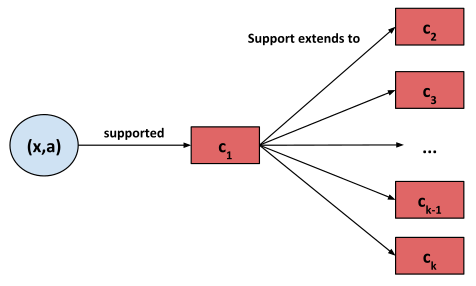
\includegraphics[width=8cm]{img/maxRPWC}
    \caption{maxRPWC}
\end{figure}

\subsubsection{Example}
\begin{figure}[!h]
\begin{tikzpicture}
    \node (A) {D(x) = \{0, 1\}};
    \node (B) [right=2cm of A] {D(y) = \{1, 2\}};
    \node (C) [right=2cm of B] {D(z) = \{1, 2\}};

    \node (D) [below right=1cm and 1cm of A] {$c_1$: x = |y-z|};
    \node (E) [below right=1cm and 1cm of B] {$c_2$: y $\neq$ z};
\end{tikzpicture}
\caption{Example CSP GAC but not maxRPWC}
\end{figure}

\begin{itemize}
    \item The support for (x,0) in $c_1$ are ((y,1), (z,1)) and ((y,2),(z,2))
    \item but those supports are not extensible to $c_2$
    \item[$\to$] (x,0) will never be part of a solution
\end{itemize}

\section{Consistencies/Propagations algorithm and constraints}

\begin{figure}[!h]
    \centering
    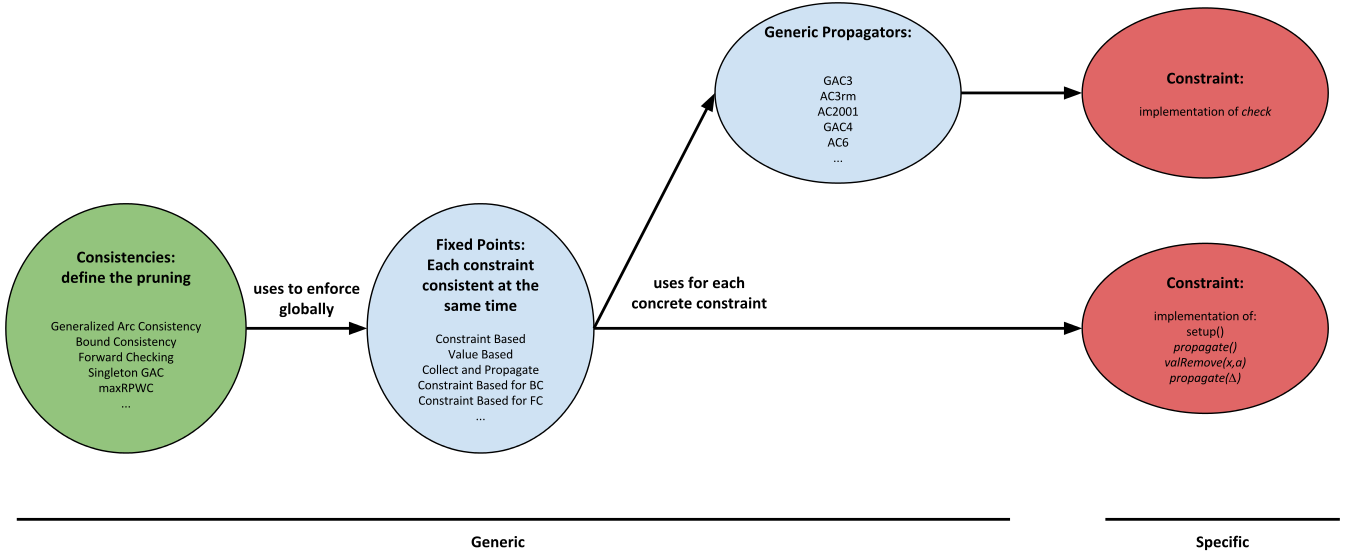
\includegraphics[width=\linewidth]{img/consistency-propagation.png}
    \caption{Link}
\end{figure}

\subsection{Mixing constraint}

The idea is to mix for different constraints : different consistencies and different fixed points

\begin{tabular}{m{1cm}cm{6cm}cm{6cm}}
    \textbf{Global fixed point}
    & = &
    \begin{itemize}
        \item ensuring each queue ($C_{CB}, C_{CV}, C_{CB-BC}, CP_{CB-FC}$) is empied
        \item ensuring impacted constraints put on the right queue
    \end{itemize}
    & \begin{tikzpicture}
        \draw[->] (0,0) edge node[above] {At the end} (1,0);
    \end{tikzpicture}
    &
    \begin{itemize}
        \item each constraint respects its consistency
        \item all at the same time
    \end{itemize}
\end{tabular}


\subsection{Mixing in practice}
\begin{enumerate}
    \item Constraints register to particular events on the domains/variables :
        \begin{itemize}
            \item a \textbf{value} has been removed (\textit{VB or collect \& propagate})
            \item the \textbf{domains} have been changed (\textit{CB})
            \item the \textbf{bounds} of the domains have changed (\textit{CB for BC})
            \item a variables is \textbf{assigned} (\textit{CB for FC})
        \end{itemize}

    \item When event occurs in a domain/variable :
        \begin{itemize}
            \item constraints put on the right queue and fixed point resumed
            \item makes the bridge between different queues
        \end{itemize}
\end{enumerate}



\section{Search}

\paragraph{Search tree} is defined by
\begin{itemize}
    \item One CSP
    \item Branching
    \item Variable/value selection heuristic
    \item Exploration strategy
\end{itemize}

\paragraph{Tree} The tree is constructed during exploration and only the current
node in memory (DFS). The alternative decisions is memorized.

\paragraph{Node expansion}
Subdivision of a CSP into smaller CSP such that the union of the small CSP
is equivalent to the original.


\subsection{Depth first backtraking search}

\begin{itemize}
    \item Based on:
    \begin{enumerate}
            \item \textbf{stack of sets of decision}
            \item \textbf{stack of restoration states}
        \end{enumerate}
    \item Backtracking restores:
        \begin{enumerate}
            \item Variables/domains
            \item Constraints
            \item Backtracked structures (ex: fistSupport)
        \end{enumerate}
\end{itemize}

\begin{lstlisting}[caption=Depth First backtracking search]
while (! decisionStack.isEmpty) {
    val decisionsOfNode = decisionStack.pop()

    val decision = decisionsOfNode.pop()
    if( decision.hasNext() )
        pushState()

    applyDecision(decision)

    if (!isFailed() ){
        val isExpandable = expand(branching)
        if (! isExpandable) {
            solFound()
            popState()
        }
    } else {
        popState()
    }
}
\end{lstlisting}

\subsubsection{Trailing}
In opposition to copying the node in order to perform backtracking,
trailing only store the \textbf{modification}.

\paragraph{Trail level}
Trailed operations are marked with an integer which is increase!

\paragraph{Restoring} undo all operations with trail level greater than
desired set the trail level to desired one.


\subsection{Branching strategy}

\paragraph{Completeness}: a branching strategy is \textbf{completeness}
if the union of the child CSPs is the parent CSP

\subsubsection{Strategies}
\begin{tabular}{m{6cm}m{6cm}}
    \begin{itemize}
        \item binary labelling
    \end{itemize}
    &
    \begin{tikzpicture}[scale=0.7]
        \node[] {\scriptsize$P_1$} child{ node[] {\scriptsize$P_2$}
        edge from parent node[above, left] {$x_1 = a$}}
        child { node[] {\scriptsize$P_3$}
        edge from parent node[above, right] {$x_1 \neq a$}};

    \end{tikzpicture}
    \\
    \begin{itemize}
        \item n-ary labelling
    \end{itemize}
    &
    \begin{tikzpicture}[scale=0.7]
        \node[] {\scriptsize$P_1$} child{ node[] {\scriptsize$P_2$}
        edge from parent node[above, left] {$a$}}
        child { node[] {\scriptsize$P_3$}
        edge from parent node[above, right] {$b$}}
        child { node[] {\scriptsize$P_4$}
        edge from parent node[above, right] {$c$}}
        child { node[] {\scriptsize$P_4$}
        edge from parent node[above, right] {$d$}};

        \node at (-3,-1) {\scriptsize $x_1 =$};
    \end{tikzpicture}
    \\
    \begin{itemize}
        \item domain splitting
    \end{itemize}
    &
    \begin{tikzpicture}[scale=0.7]
        \node[] {\scriptsize$P_1$} child{ node[] {\scriptsize$P_2$}
        edge from parent node[above, left] {$x_1 \geq t$}}
        child { node[] {\scriptsize$P_3$}
        edge from parent node[above, right] {$x_1 < t$}};

    \end{tikzpicture}
    \\
\end{tabular}

\subsubsection{Heuristics}

\begin{enumerate}
    \item Select a variable
    \item Ordering the values
\end{enumerate}

Take care than the first decisions have a high impact!

\subsubsection{Variable ordering heuristics}

Variables heuristic impact the \textbf{number of node} but not the numbers
of leaves.

\paragraph{First fail principle}: choose first a variable that is more likely to fail
(Consider the most difficult parts of the CSP first)

\begin{itemize}
    \item[No first-fail]
    \item \textbf{Random} : select variable randomly (\textit{Usefull in cases of restarts})

    \item \textbf{Lex} : lexicographic order (\textit{static})

    \item[Can first-fail]
    \item \textbf{Predefined order}: predefined once before search
        (\textit{static})

    \item[First-fail]

    \item \textbf{Deg heuristic}: select the variable with the \textit{highest}
        number of constraint involving.
        (\textit{static heuristic})

    \item \textbf{DDeg heuristic}: select the variable with the \textit{highest}
        number of constraint involving, only counting constraint with more than
        two uninstantiated variables
        (\textit{dynamique heuristic})

    \item \textbf{wDeg heuristic}: select the variable with the \textit{highest}
        $\sum$ weights of constraints involving.
        (\textit{dynamique heuristic})

        $\to$ Give a adapative weight to each constraint which depend on the
        search node and the previously visited nodes.

    \item \textbf{Activity based variable ordering}: record the activity A(x) of
        each variable x.

        Select the most active variable which is the most harder.

        \paragraph{At each node}
        \begin{itemize}
            \item reduce activity of all variable : $A(x) =  A(x) . \gamma, \quad (0 < \gamma < 1$)
            \item increase activity of active variable : $A(x) = A(x) + 1, \quad$
                if D(x) has been reduced
        \end{itemize}
\end{itemize}

%TODO slide 48 - search

\subsubsection{Value ordering heuristics}

\paragraph{Best first principle}: Choose first a value that is more likely to succeed

\begin{itemize}
    \item[No best-first]
    \item \textbf{Random} : select value randomly
    \item \textbf{Lex} : lexicographic order (\textit{static})

    \item[Best-first]
    \item \textbf{Pruning based heuristic}: select the value which induced
        the minimum pruning or largest minimun pruning.

        $\to$ Give a adapative quantities to each constraint which depend on the
        search node and the previously visited nodes.

    \item \textbf{Number of solutions based heuristic}: select the value
        which has the maximun number of solutions.

        $\to$ Give a adapative quantities to each constraint which depend on the
        search node and the previously visited nodes.

    \item \textbf{Activity based value ordering}: record the activity A(x) of
        each value (x, a).

        Select the less active variable which is the less pruning.

        \paragraph{At each node where x=a tried}
        \begin{itemize}
            \item $A(x=a) = A(x=a) . (a - \alpha) + \alpha . k , \quad (0 < \alpha \leq 1)$

                k = number of active variable when enforcing x=a
        \end{itemize}
\end{itemize}

\subsection{Exploration strategies}

\begin{itemize}
    \item \textbf{DFS}: fully trust the variable/value heuristic.
        $\to$ \textit{limited information}

        \paragraph{Note:} errors at the top of the tree is \textbf{expensive}


    \item \textbf{Discrepancy Search}: do not trust too much the heuristics.
        Take the right branch correspond to not trusting the value heuristic!
        (n-ary or binary branching)

        \paragraph{Discrepancy}: number of times right branch chosen in
        a path from root to the node.

        $\to$ The nodes are visites in increasing discrepancy order

        \begin{figure}[!h]
            \centering
            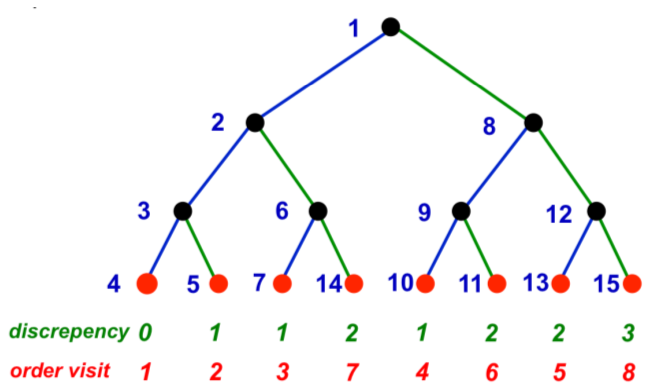
\includegraphics[width=8cm]{img/discrpancy.png}
            \caption{Discrepancy search}
        \end{figure}

        \begin{itemize}
            \item[+] better diversification and alleviate the cost
                of early mistakes
            \item[-] Space complexity exponential in worst case
        \end{itemize}

    \item \textbf{Restart}: Search can be restarted after a certain limit
        (\textit{time, number of fails, number node visited,\ldots}) with a different
        variable/value heuristic.

        \begin{description}
            \item[Adaptive heuristics] can us information from multiple runs.
            \item[Completness] if limite large enough and limit increased between restarts
        \end{description}
        \begin{itemize}
            \item[+] diversification and alleviate the cost of early mistakes
            \item[$\to$] useful for heavy tailed problems (ex: sport scheduling)
        \end{itemize}

\end{itemize}

\section{Global constraints}

\subsection{Example}

\begin{itemize}
    \item \texttt{allDifferent($[x_1,\cdots, x_r]$)}

    \item \texttt{Element($Array, index, value$): $Array(index) == value$}

    \item \texttt{GCC($[x_1,\cdots, x_r]$, $[v_0,\cdots, v_k]$, $[m_0,\cdots, m_k]$,
        $[M_0,\cdots, M_k]$)} : $v_i$ must appear between $m_i$ and $M_i$

    \item \texttt{table($[x_1,\cdots, x_r]$, $tab_{combinations}$)}

    \item \texttt{sum($[x_1,\cdots, x_]$, $sum$)}

    \item \texttt{sumLe($[x_1,\cdots, x_]$, $upperBound$)}

    \item \texttt{knapsack($[x_1,\cdots, x_r]$, $Profit[r]$, $Weight[r]$, $p$, $w$)}
\end{itemize}


\subsection{Advantage}
\begin{itemize}
    \item Increasing expressivity of CP
    \item Pruning strength because the propagation considered constraint in isolation
        but global constraint is like \textbf{a set of constraint}
    \item Pruning efficiency because no fixed point between small constraints
        but a more flobal reasoning
\end{itemize}

\subsection{Decomposition}
A set of constraints $S$ is called the decomposition of $g$ iff :
$$ \forall D(X): sols(X, D(X), \{g\}) = sols(X, D(X), S)$$

\paragraph{GAC} GAC pruning equivalent in $S$ and $g$ iff the constraint
graph of the D is \textbf{acyclic}.

Otherwise, GAC pruning stronger in global constraint

\begin{itemize}
    \item GAC on decomposition : supports(s) for each literal on each constraints
        \textbf{separately}
    \item GAC on global constraint: global support(s) for each literal on global constraint
\end{itemize}


\paragraph{FC} FC pruning stronger in the decomposition


\subsection{AllDifferent constraint}

GAC pruning for \texttt{allDifferent($[x_1,\cdots, x_r]$)} use a value graph :
\begin{itemize}
    \item one node for each variable $x_1,\cdots, x_r$
    \item one node for each value in $\cap D(x_i)$
    \item one edge between $x_i$ and $a$ if $a \in D(x_i)$
    \item[Note:] bipartite graph
\end{itemize}

\subsubsection{Matching}
A matching is a \textbf{set of edgges} such that no edge share
a same node.

\begin{itemize}
    \item Size matching = \# edges
    \item Maximum matching = largest size
    \item Maximum size = \# variables
\end{itemize}

\begin{description}
    \item \texttt{AllDifferent($[x_1,\cdots, x_r]$)} satisifiable iff
        $\exists$ matching of the value graph covering $x_1,\cdots, x_r$ (=
        matching of maximum size)
    \item M is a maximum matching iff no augmenting
        path exists
\end{description}

\subsubsection{Finding a maximum matching}

\begin{enumerate}
    \item Start with any matching (e.g. empty matching)
    \item Iteratively improve the matching with \textbf{augmenting path}

        \paragraph{Augmenting path}
        \begin{itemize}
            \item Edge in M : variables $\to$ values
            \item Other : values $\to$ variables

            \item[$\Rightarrow$] An augmenting path is a \textbf{directed path}
                from a uncovered value to an uncovered variable.

                Use DSF or BFS
        \end{itemize}

        \begin{figure}[!h]
            \centering
            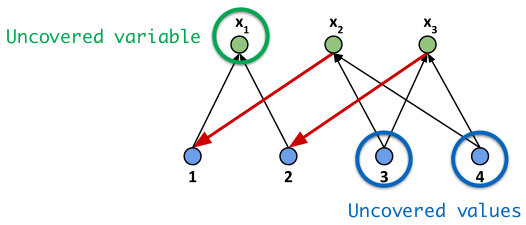
\includegraphics[width=8cm]{img/augmenting-paths.png}
            \caption{Augmenting paths}
        \end{figure}

    \item Stop when no more augmenting paths
\end{enumerate}

\subsubsection{GAC}

\begin{description}
    \item \texttt{AllDifferent} is \textbf{GAC} iff all edge belong to
        a maximun matching covering all the variables
\end{description}

\begin{itemize}
    \item \textbf{Alternating path}

    \item \textbf{Alternating cycle}

\end{itemize}

\paragraph{Filtering}

\begin{enumerate}
    \item Find a maximun matching M
    \item if M.size != \#variables : \textcolor{red}{Fail}

    \item Find all edges belonging to an even \textbf{length alternating
        path} startint at a uncovered node (DFS or BDS)

        \paragraph{Alternating path}: start at an uncovered node and
        switch the edges in/out the matching. Change values
        of variables to stays maximum with different edges.

        \begin{figure}[!h]
            \centering
            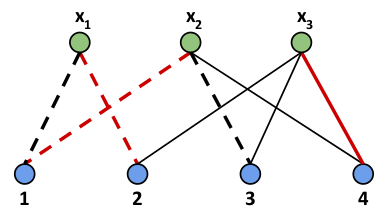
\includegraphics[width=8cm]{img/alternating.png}
            \caption{Alternating paths}
        \end{figure}

    \item Find all edges belonging to \textbf{alternating cycle} which
        correpons to the strongly connected components in the directed value
        graph

        \paragraph{Alternating cycle}: switch the edges in/out the matching.
        Exchange values of variables to stays maximum with different edges.

    \item Remove all edges/literals not in M and not found
\end{enumerate}

\paragraph{Incrementality of the filtering}
The value graph and maximum matching is keep in memory between calls to propagator.

\begin{tabular}{cm{12cm}}
When called
&
\begin{enumerate}
    \item Remove esdge not present anymore
    \item recompute maximum matching if necessary
    \item recompute GAC edges
\end{enumerate}
\end{tabular}

\subsection{Sum constraint}

\subsubsection{NP-Hard}
Gac for a sum constraint is NP-Hard :

\paragraph{Proof} reduction of subset-sum to GAC for Sum
\begin{itemize}
    \item subset-sum: a NP-Hard problem for integer set ($S=\{a_1,\cdots, a_r\}$),
        does any non-empty subset of S sums to 0?

    \item reduction to GAC for Sum:
        \begin{lstlisting}[mathescape]
variables  $x_i$ with domains $\{0, a_i\}$
GAC on sum($[x_1,..., x_r], 0$)

if $D(x_i) = \{0\} \forall x_i$ : answer no
else: answer yes
\end{lstlisting}
\end{itemize}

\paragraph{Consequences} GAC propagator for sum is exponential (unless P=NP), so
the propagator is usually done with \textbf{Bound Consistency}

\subsubsection{Bound consistency}
\begin{lstlisting}
propagate(){
    $\Delta = \emptyset$
    for( x $\leftarrow$ scope) {
        new_min = k - ($\sum_{(y \in scope, y \neq x)} y.max$)
        for( a $\leftarrow$ D(x) if a < new_min)
            $\Delta$ += (x, a)

        new_max = k - ($\sum_{(y \in scope, y \neq x)} y.min$)
        for( a $\leftarrow$ D(x) if a > new_max)
            $\Delta$ += (x, a)
    }
    return $\Delta$
}
\end{lstlisting}

\subsection{Global Cardinality constraint}

GAC filtering for \texttt{GCC($[x_1,\cdots, x_r]$, $[v_0,\cdots, v_k]$, $[m_0,\cdots, m_k]$,
$[M_0,\cdots, M_k]$)} use the \textbf{value network} :

\begin{tabular}{m{8cm}m{8cm}}
\begin{itemize}
    \item \begin{tabular}{l}
            one node per value\\
            one node per variable \\
            edge from values to variables \\
        \end{tabular}
    \item \begin{tabular}{l}
            one special node $s$ (source)\\
    one special node $p$ (target) \\
\end{tabular}
    \item Edges : $s \to values \to variables \to p \to s$
\end{itemize}
&
    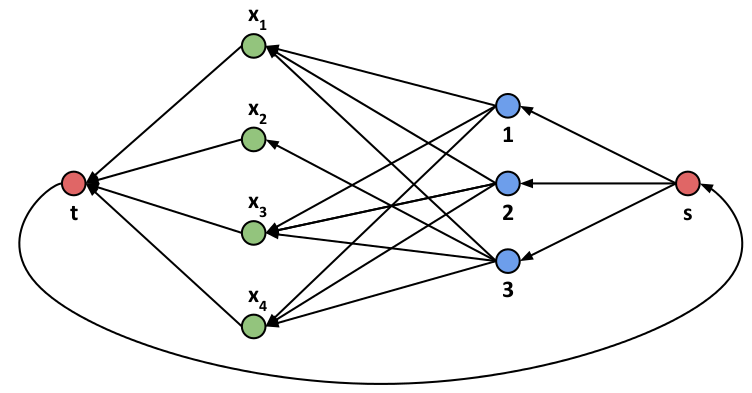
\includegraphics[width=8cm]{img/valuenetwork.png}
\end{tabular}

\subsubsection{Flow}

We can use flow through the value network to ensure some constraint
(\textbf{flow requirements [low, cap]}).

\begin{tabular}{m{8cm}m{8cm}}
\begin{itemize}
    \item[$s \to v_i$]: $[m_i, M_i]$
    \item[$\Rightarrow$] GCC constraint (cardinalities)
    \item[$v_i \to x_k$]: $[0, 1]$
    \item[$x_i \to t$]: $[1, 1]$
    \item[$\Rightarrow$] Exactly one value per variable
    \item[$t \to s$]: $[r, r]$
\end{itemize}
&
    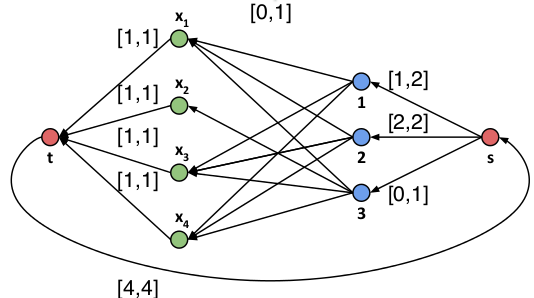
\includegraphics[width=8cm]{img/flow.png}
\end{tabular}

\begin{description}
    \item[Flow conservation]: for a graph $G = (N, E)$ :
        $$ \forall n \in N, \sum_{(n', n) \in E)} f(n', n) = \sum_{(n, n') \in E)} f(n, n')$$

    \item[Feasible flow]: gives a flow value to each edge, respects
requirement and conservation

\item[Satisfiable] For a GCC constraint c: c is satisfiable iff $\exists$ a
feasible flow in the value network of c

\end{description}

\subsubsection{Filtering procedure}

\begin{enumerate}
    \item Start with zero flow: $\forall (x, y),  f(x, y) = 0$
    \item[Check feasible]
    \item If no edge with $f(x, y) < low(x, y)$ : \textbf{feasible flow} found
    \item Else:
        \begin{enumerate}
            \item Find a \textbf{augmenting path} from y to x in the
                \textbf{residual graph} (not using $(y, x)$)
            \item Augment the flow
            \item If no augmenting path: no feasible flow exist
        \end{enumerate}
    \item[Filtering]
    \item Remove (var, val) if
        \begin{itemize}
            \item f(val, var) = 0
            \item val and var not in the same strongly connected component
                in the residual graph
        \end{itemize}
\end{enumerate}

\paragraph{Incrementality of the filtering}
The value network and feasible flow is keep between two calls.

\begin{tabular}{cm{12cm}}
When called
&
\begin{enumerate}
    \item Remove edge not present anymore
    \item recompute feasible flow if necessary
    \item recompute non-GAC edges
\end{enumerate}
\end{tabular}


\paragraph{In a value network}: no augmenting path from var to val iff
var and val not in the same strongly connected component in
residual graph

\paragraph{In a feasible flow $f$ in the value network}:

\begin{tabular}{m{7cm}cm{3cm}cm{3cm}}
    if f(val, var) = 0 and no augmenting path from var to val
    & $\leftrightarrow$ &
    f(val, var) is maximum 0
    & $\leftrightarrow$ &
    (var, val) is not GAC
\end{tabular}

\subsubsection{Residual graph} For a graph $G=(N, E)$ and a flow $f$,
the residual graph $R=(N, E')$ such that :
\begin{itemize}
    \item $E' = A^+ \cup A^-$ :
        \begin{description}
            \item if $f(x, y) < cap(x, y)$ : $(x, y) \in A^+$ with requirement
                [0, cap(x, y) - f(x, y)]

            \item if $f(x, y) > low(x, y)$ : $\color{red}(y, x)$ $ \in A^-$ with requirement
                [0, f(x, y) - low(x, y)]
        \end{description}
\end{itemize}

\begin{figure}[!h]
    \begin{tabular}{cc}
        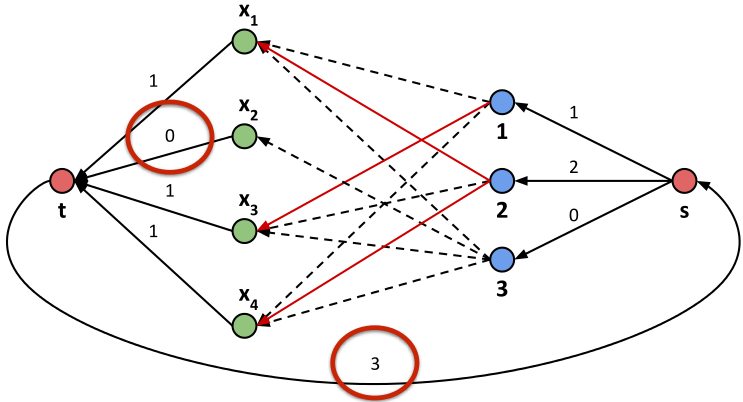
\includegraphics[width=0.5\linewidth]{img/residual1.png}
        &
        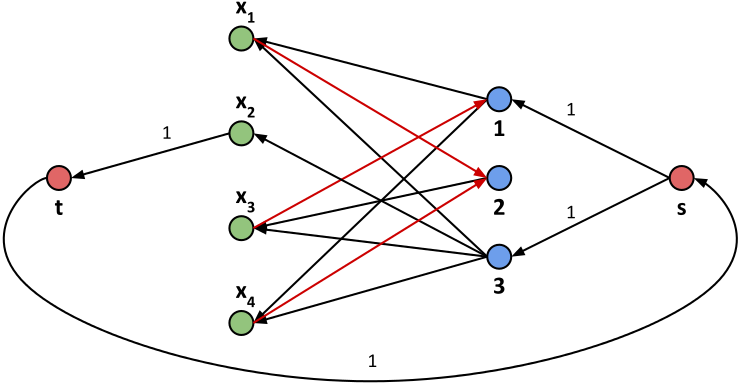
\includegraphics[width=0.5\linewidth]{img/residual2.png}
        \\
        The flow $f$ is represent in this picture &
        The corresponding residual graph \\
    \end{tabular}
    \caption{Residual graph}
\end{figure}

\subsubsection{Augmenting path} From augmenting path $p$
\begin{itemize}
    \item $val = min_{(x,y) \in p} cap(x, y)$
    \item For all edge in $A^+$ : augment flow by val
    \item For all edge in $A^-$ : decrement flow by val
\end{itemize}

\begin{figure}[!h]
    \begin{tabular}{cc}
        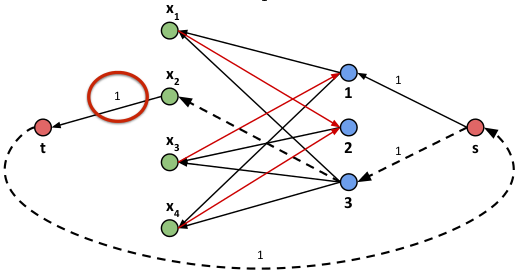
\includegraphics[width=0.5\linewidth]{img/augmenting1.png}
        &
        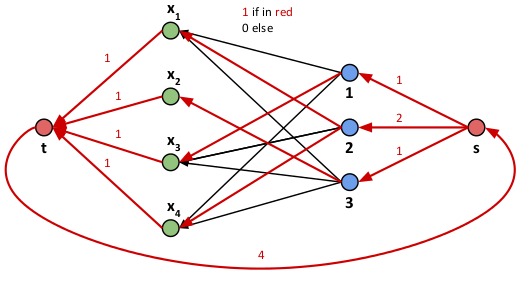
\includegraphics[width=0.5\linewidth]{img/augmenting2.png}
        \\
        Residual graph with augmenting path&
        The flow $f$ at the end\\
    \end{tabular}
    \caption{Augmenting path}
\end{figure}



\subsection{Table constraint}

The table correspond to a table of tuple of value accepted.

$\to$ Literal (x,a) supported if 
\begin{center}
$\exists$ tuple \textbf{valid} (= all its
value are in the domain) in the table where x=a
\end{center}


\begin{itemize}
    \item \textbf{Simple tabular reduction}: When a tuyple is found valid,
        all its value are supported. If tuple is invalid, he is removed from the
        table.

        \begin{center}
            In a table on (x,y,z) if tuple (a,b,c) valid $\to$
            (x,a), (y,b) and (z,c) supported
        \end{center}


        \begin{lstlisting}[mathescape]
STR(X,table){
     supported = $\emptyset$
     for(t $\leftarrow$ table){
        // if tuple is valid
         if($\forall x_i : x_i$.hasValue(t(i))){
            // literal collected
             for($x_i \leftarrow X$){
                 supported += ($x_i ,t(i)$)
             }
         }
        // removed tuple
        else
             table.remove(t)
     }
    // unsupported literal returned
     return D(x)/supported
}
\end{lstlisting}

    \item \textbf{Incrementality of STR}: The removed tuple are
        removed by a way incrementaly. It's means that when a tuple is
        removed, he is not inspected in future executions!

        $\to$ Table has to be backtracked.

    \item \textbf{Efficiently backtrackable table}: The backtracking need
        to be efficient, so we can't backtracking the whole table because
        it's costly.

        The solution is to use a \textit{Sparse set} to represent the table
        which only need to backtracked \textbf{one integer}.

\end{itemize}

\subsubsection{Sparse set data structure}

\begin{tabular}{m{10cm}m{1.5cm}m{1.5cm}m{1.5cm}}
\begin{itemize}
    \item Table is partitionned into two set (present tuple
        and removed tuple).

    \item When a tuple is removed, it is exchanged with the tuple
        in position size and size decremented.

    \item On backtracking, we restore size $\to$ restore removed tuples
        at different positions in the table.
\end{itemize}
&
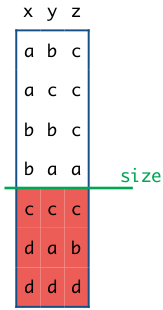
\includegraphics[width=1.5cm]{img/sparse.png}
&
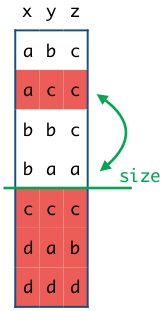
\includegraphics[width=1.5cm]{img/sparse2.png}
&
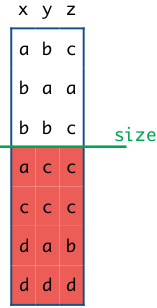
\includegraphics[width=1.5cm]{img/sparse3.png}
\end{tabular}


\paragraph{Dynamic table}
The dynamic table is \textbf{not represented}!

\begin{itemize}
    \item \texttt{Map()} such that $Map(i)$ =
        position of tuple $i$ in the dynamic table

    \item \texttt{Dyn()} such that $Dyn(i)$ = tuple indice
        in position i
\end{itemize}

\subsubsection{Propagator}
Many propagator for TC :
\begin{itemize}
       \item Multi-valued decision diagram (MDD)
       \item Trie-based algorithm
       \item Optimal value-based AC5TCOpt-Sparse
       \item Optimal value-based STR3
       \item \ldots
\end{itemize}

\section{Optimization}

A COP is described with \texttt{(X, D, C, O)}.

\paragraph{Over-constrained problem}
In some case, there is no solution for the problem\ldots In this case, we
can put some \textit{soft constraint} which can be violated with
a associated \textbf{cost}.

\subsection{Complete optimization}

\begin{enumerate}
    \item \textbf{Branch and bound}: for an objective function $O$ (arithmetic expression).

        At each solution $s$, add a constraint :
        \begin{itemize}
            \item min: $O < \bigoh(s)$
            \item max: $O > \bigoh(s)$
        \end{itemize}

        and stop when no more solutions.

        \paragraph{Optimality} proof at the last solution found

        \paragraph{Too hard problem}:
        \begin{itemize}
            \item Need to define a time/backtrack limit
            \item B\&B doesn't show good diversification
            \item can fail to find a single solution
        \end{itemize}

    \item \textbf{Iterative optimization}: need to compute a
        \begin{tabular}{r}
            lower bound \\
            upper bound
        \end{tabular}.

        \begin{enumerate}
            \item add \begin{tabular}{r}
                    $0 \leq lb$ \\
                    $0 \geq ub$ \\
                \end{tabular}
            \item if a solution : it's optimal
            \item if not : \begin{tabular}{r}
                    increase \\
                    decrease \\
                \end{tabular}
        \end{enumerate}

        \paragraph{Too hard problem}: iterative optimization
        doesn't find any solution
\end{enumerate}

\paragraph{Completeness} is a great \textbf{asset} but sometimes it is too
costly!

\subsection{Constraint based local search}

\begin{table}[!h]
    \centering
\begin{tabular}{m{7cm}|m{7cm}}
    \multicolumn{1}{c}{CP} & \multicolumn{1}{c}{CBLS} \\
    \hline
    \begin{itemize}
        \item Use constraints
        \item Constructive approach
        \item Complete search
        \item Solving model with branch and propagate
    \end{itemize}
    &
    \begin{itemize}
        \item Use constraints
        \item Pertubative approach
        \item Imcomplete search
        \item Solving model with neighborhoods
    \end{itemize}
    \\
    Find best solution but can take too much time
    &
    Find a good solution quickly\\
\end{tabular}
\caption{Constraint programming VS constraint based local search}
\end{table}

CBLS :
\begin{itemize}
    \item Always has a \textbf{current solution} which is not optimal (or not know to be)
    \item \textbf{Iteratively improve} the current solution :
        \begin{enumerate}
            \item define the neighborhood of the current solution
            \item select one of the neighbors
            \item choice to accept it as the new current solution
        \end{enumerate}

    \item Additionnal help from the model :
        \begin{itemize}
            \item violations of soft constraints
            \item invariants
            \item differentiable constraints
            \item differentiable objective function
            \item propagation in hard constraint and objective function
        \end{itemize}
\end{itemize}

%TODO : invariant + differentiable object

\paragraph{Local optima}
We search for \textbf{global optima} but local search may
lead to local optima due to the local nature of LS...

\paragraph{Heuristic}

\begin{itemize}
    \item chooses next solution in neighborhood based on local information
(memoryless)
    \item[$\to$] drives the search toward \textbf{local} optima
\end{itemize}

    \paragraph{Meta-heuristic}

    \begin{itemize}
    \item collect information on the execution
    \item[$\to$] drives the search toward \textbf{global} optima
    \end{itemize}

\subsection{CP-LS}

\begin{tabular}{m{0.5cm}m{6cm}m{0.5cm}m{0.5cm}m{6cm}}
LS &
\begin{itemize}
\item efficient to find good solution quickly
\item diversify efficiently
\end{itemize}
& + & CP &
\begin{itemize}
\item Complete
\item Propage information
\end{itemize}
\end{tabular}

\paragraph{Hybridizations}
\begin{itemize}
    \item \textbf{Sequential}
        \begin{description}
            \item[] \begin{tabular}{m{3cm}m{11cm}}

                    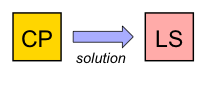
\includegraphics[width=3cm]{img/cpls1.png}
                    &
                    \begin{enumerate}
                        \item CP compute an initial solution non-optimal (respects hard-constraint)
                        \item LS start with this inital solution
                    \end{enumerate}
                \end{tabular}
            \item[] \begin{tabular}{m{3cm}m{11cm}}

                    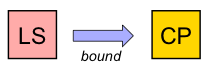
\includegraphics[width=3cm]{img/cpls2.png}
                    &
                    \begin{enumerate}
                        \item LS compute an initial solution non-optimal (respects hard-constraint)
                        \item CP used initial bound (from solution) and prove optimality
                    \end{enumerate}
                \end{tabular}

        \end{description}


    \item \textbf{Parallel cooperation}
        \begin{description}
            \item[] \begin{tabular}{m{3cm}m{11cm}}

                    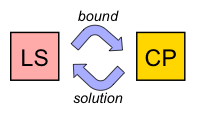
\includegraphics[width=3cm]{img/cpls3.png}
                    &
                    \begin{enumerate}
                        \item When LS improves a solution : new bound for CP
                        \item When CP find a solution: send it to LS for improvement
                            or diversification
                    \end{enumerate}
                \end{tabular}
        \end{description}

    \item \textbf{Mast-Slate cooperation}
        \begin{description}
            \item[] \begin{tabular}{m{1.5cm}m{12.5cm}}
                    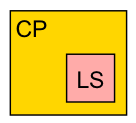
\includegraphics[width=1.5cm]{img/cpls4.png}
                    &
                    Integrated LS within a CP search :
                    \begin{enumerate}
                        \item LS improves solution found by CP
                        \item LS repairs inconsistent partial solution
                    \end{enumerate}
                \end{tabular}
            \item[] \begin{tabular}{m{1.5cm}m{12.5cm}}
                    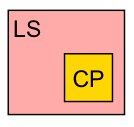
\includegraphics[width=1.5cm]{img/cpls5.png}
                    &
                    Integrated CP within a LS search :
                    \begin{enumerate}
                        \item CP used to define and explore neighborhoods
                            \paragraph{Neighborhood size threshold}
                            \begin{itemize}
                                \item large neighborhoods : small path to optimum but
                                    costly to explore
                                \item small neighborhood : long path to optimum but
                                    cheap to explore
                            \end{itemize}

                        \item[$\to$] CP can be used to explore efficiently large
                            neighborhoods

                    \end{enumerate}
                \end{tabular}
        \end{description}
\end{itemize}

\subsection{Large Neighborhood Search}

The diversification is the most weakness of CP for hard COPs.
The idea of LNS is stuck for too long $\to$ jump in the search space!

\begin{tabular}{m{10cm}m{6cm}}
    At each step :
    \begin{itemize}
        \item A portion of the variables is selected (=\textbf{fragment})
            and are relaxed to the \textbf{initial domain}
        \item The oter variables are frozen to their value in the current solution
        \item A limited CP search \textbf{improving solutions}
    \end{itemize}
    &
    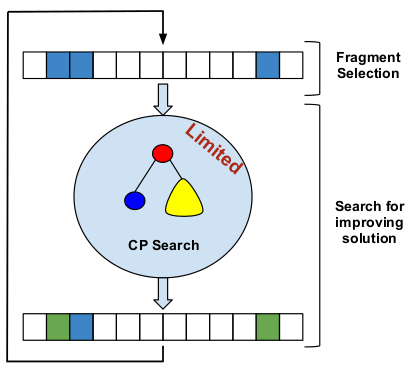
\includegraphics[width=6cm]{img/lns.png}
\end{tabular}

\paragraph{Advantages}
\begin{itemize}
    \item Good diversification if fragment well chosen
    \item Intensification with CP search
    \item No meta-heuristic needed
    \item No need to design complex feasible neighborhoods because CP
        is in charge of feasibility
    \item Scalability of LS
    \item Efficient exploration of neighborhoods with CP
\end{itemize}


\subsubsection{Designing LNS}
Parameters of LNS :
\begin{itemize}
    \item \textbf{Fragment size} and \textbf{time/backtrack limit}:
       strongly linked parameters because
       \begin{enumerate}
           \item fragment size determines neighborhood size
           \item limit determine the maximal effort to explore
       neighborhood.
       \end{enumerate}

       \paragraph{Note:} a good LNS should never be stopped only by the limit\ldots

       \paragraph{Adaptive versions}:
       \begin{enumerate}
           \item Fix a time/backtrack limit
           \item if neighborhood fully explored $\to$ increase fragment size
           \item else: decrease fragment size
       \end{enumerate}

    \item \textbf{fragment selection} (can be combined).

        Should contain important variables and related variables.

        \begin{itemize}
            \item \begin{tabular}{m{3cm}m{10cm}}
                    Random selection &
                \begin{itemize}
                    \item Surprisingly good
                    \item Generic
                    \item Excellent diversification
                    \item Intensification from CP search
                \end{itemize}
            \end{tabular}

        \item \begin{tabular}{m{3cm}m{10cm}}
                    Specific selection &
                \begin{itemize}
                    \item Only for one problem
                    \item Use knowkedge of the problem to select variables
                    \item Usually randomized to some extend
                \end{itemize}
            \end{tabular}
        \end{itemize}

\end{itemize}

%TODO: example


\section{Vehicle Routing problem}

NP-hard problem which is a optimization problem.

\subsection{Definition}
\begin{itemize}
    \item For each customer (quantity required, position, cost and time to travel
to eahc customer)
    \item For vehicles (number, capacity for each)
    \item For each route, there is a maximum time
    \item[$\to$] We must find the route visiting all customer
            respecting constrains and minimizing the cost
\end{itemize}

\subsubsection{Objective function}
Objective function can include :
\begin{itemize}
    \item A number of vehicles \begin{tabular}{l}
            fixed \\ separate problem \\ part of objective function
        \end{tabular}

    \item A costs \begin{tabular}{l}
            same for each vehicle \\ depend on truck/staff
        \end{tabular}

    \item Total distance and maximum distance for truck

    \item Total time and maximum time for a route
\end{itemize}

\subsubsection{Constraints}

\begin{itemize}
    \item Time window constraints
    \item Delivery mode (truck start/end route at a depot)
    \item (in)compatibility constraints \begin{tabular}{l}
            between a sets of goods (food - toxic product)\\
            between goods and vehicle (food in refrigerated truck)
        \end{tabular}
    \item Fatigue rules and driver breaks
    \item Modular vehicle
    \item 2D/3D loading constraints (goods must be placed in the inverse visit order)
\end{itemize}

\subsubsection{Variant} profitable VRPs where
\begin{itemize}
    \item some visits are optional
    \item visiting clients brings profit and has cost
    \item[$\to$] maximize profit and route vehicles
\end{itemize}

\subsection{Solving Rich VRP}

\begin{itemize}
    \item By \textbf{Complete techniques}

        $\to$ optimal solution but costly
    \item by \textbf{Heuristic techniques} (like Local search, generic algorithm,\ldots)

        $\to$ non-optimal solution but quickly
    \item[Problem]:
\end{itemize}

\subsubsection{Model for a Rich VRP (with hard side constraints)}

\paragraph{Variable}:

\begin{tabular}{rrr}
    \begin{minipage}[b]{0.3\linewidth}

    \begin{tabular}{m{\linewidth}}
        \textbf{Customers}\\
        \hline
        $n$ customers (1..n)\\
        Demand: $Dem_{i, k}$ for good k \\
        Value: $V_i$\\
        Time win: $[E_i, L_i]$\\
        Service time: $S_i$\\
        Distance (i $\to$ j): $D_{i, j}$\\
        Time (i $\to$ j): $T_{i, j}$\\
        \\
        \textbf{Truck}\\
        \hline
        q(i,k): quantity of good k after customer i
    \end{tabular}
\end{minipage}
&
\begin{minipage}[b]{0.3\linewidth}
    \begin{tabular}{m{\linewidth}}
        \textbf{Vehicle}\\
        \hline
        $m$ vehicles\\
        Capacity: $Q_{i, k}$ for good k\\
        One route per vehicle\\
        One depot\\
        Vechicle start/end to depot\\
        \\
        \textbf{Time Window}\\
        \hline
        a(i): arrival time customer $i$\\
        serv(i): service start customer $i$\\
        dep(i): departure time customer $i$\\
    \end{tabular}
\end{minipage}
&
\begin{minipage}[b]{0.3\linewidth}
    \begin{tabular}{m{\linewidth}}
        \textbf{Route}\\
        \hline
        One truck = one route (1\ldots m)\\
        Route 0 for unvisited\\
        A route = \{set of visits\}\\
        \\
        \textbf{Visites}\\
        \hline
        Start/end visit route $k$ : $n+k$ and $n+m+k$\\
        Start/end visit route $0$ : $n+2m+1$ and $n+2m+2$\\
    \end{tabular}
\end{minipage}
\end{tabular}


\paragraph{Decision variable}:

\begin{tabular}{m{11cm}m{5cm}}
\begin{itemize}
    \item $succ(i) \in \{1,\cdots,n\} \cup \{n+m+1,\cdots,n+2m\} \cup \{n+2m+2\} $

        IF $i \in \{1,\cdots,n\}$
    \item $succ(i) \in \{1,\cdots,n\}$

        IF $i \in \{1,\cdots,n\} \cup \{n+1,\cdots,n+m\} \cup \{n+2m+1\}$
    \item $succ(i)=0$ for route's ends

    \item $pred(i) \in \{1,\cdots,n+m\} \cup \{n+2m+1\} $

        IF $i \in \{1,\cdots,n\}$
    \item $pred(i) \in \{1,\cdots,n\}$

        IF $i \in \{n+m+1,\cdots,n+2m\} \cup \{n+2m+2\}$
    \item $pred(i)=0$ for route's starts

    \item $route(i) = \{0,\cdots, m\}$

\end{itemize}
&
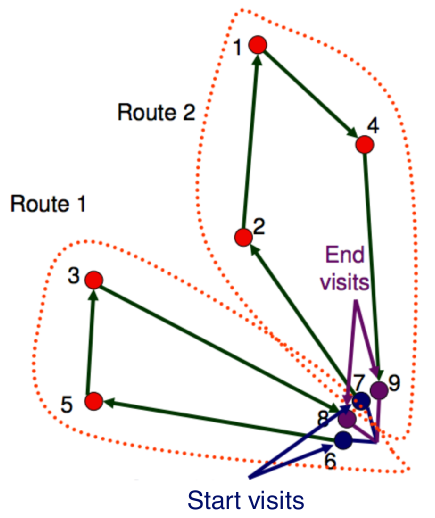
\includegraphics[width=6cm]{img/VRP.png}
\end{tabular}

\paragraph{Objective function}
$$minimize \quad \sum_{i \in \{1,\ldots,n\} \cup \{n+1,\ldots,n+m\}} C_{i, succ(i)}
+ \sum_{i \in \{1,\ldots,n\} or r(i)=0} V_i$$

= Cost of serving client + cost of no serving client

\paragraph{Constraints}:

\begin{lstlisting}[mathescape]
noCycles(succ) $\bigwedge$ noCycles(pred)

// Time
a(succ(i)) = dep(i) + $T_{i,succ(i)} \forall i \in \{1,...,n\} \cup \{n+1,...,n+m\} U \{n+2m+1\}$

serv(i) $\geq$ a(i) $\forall i \in \{1,...,n\}$
serv(i) $\geq$ $E_i \forall i \in \{1,...,n\}$
serv(i) $\leq$ $L_i \forall i \in \{1,...,n\}$
serv(i) + $S_i = dep(i) \forall i \in \{1,...,n\} $
dep(i) = 0i $\forall i \in \{n+1,...,n+m\} \cup \{n+2m+1\}$

// Load
q(succ(i),k) = q(i,k) + $Dem_{succ(i),k} \forall i \in \{1,...,n\} U \{n+1,...,n+m\} U \{n+2m+1\}$
                                         $\forall k \in \{1,...,p\}$
q(i,k) $\leq$ Q route(i),k $\forall i \in \{1,...,n\}, \forall k \in \{1,...,p\}$
q(i,k) = 0 $\forall i \in \{n+1,...,n+m\} U \{n+2m+1\}$
            $\forall k \in \{1,...,p\}$

// Consistency
succ(pred(i)) = i $\forall i \in \{1,...,n\} \cup \{n+m+1,...,n+2m\} \cup \{n+2m+2\}$
pred(succ(i)) = i $\forall i \in \{1,...,n\} \cup \{n+1,...,n+m\} \cup \{n+2m+1\}$
route(succ(i)) = route(i) $\forall i \in \{1,...,n\} \cup \{n+1,...,n+m\} \cup \{n+2m+1\}$
route(n+k) = k $\forall k \in \{1,...,m\}$
route(n+m+k) = k $\forall k \in \{1,...,m\}$
route(n+2m+1) = 0
route(n+2m+2) = 0
\end{lstlisting}

\subsubsection{Search}

%TODO

\section{Nurse Rostering problem}
\subsection{Definition}
\begin{itemize}
        \item For each nurse a qualification and some unavailable time
        \item Shift (morning/aftermoon/night), nurse work one shift a day and
            rest periods must be allocated to nurses
        \item Deman for a qualification during a shift
\end{itemize}

\subsubsection{Objective function}
Objective function can include :
\begin{itemize}
    \item feasible solution
    \item Load balancing costs
    \item Preferences of the nurses
\end{itemize}

\subsubsection{Constraints}

\begin{itemize}
    \item Meet the demand
    \item The work assignement must follow a set of rules : rules on the sequence
        of shift and repartition of rest shifts
\end{itemize}


\subsubsection{Model for NRP}

\paragraph{Variable}:

\begin{tabular}{rrr}
    \begin{minipage}[b]{0.5\linewidth}

    \begin{tabular}{m{\linewidth}}
        \textbf{Nurse}\\
        \hline
        $n$ nurses \\
        Qualification: $Q_{i, k}$ = 1 (0) if $i$ qualified (or not) for $k$\\
    \end{tabular}
\end{minipage}
&
\begin{minipage}[b]{0.5\linewidth}
    \begin{tabular}{m{\linewidth}}
        \textbf{Demand}\\
        \hline
        $D_{d, k, s}$ on day $d$, for qualification $k$ during
        shift $s$\\
        Day to plan: $nd$\\
        Diff qualif: $nk$
    \end{tabular}
\end{minipage}
\end{tabular}


\paragraph{Decision variable}:

\begin{itemize}
    \item $Shift(i,d)$ = shift for nurse $i$ on day $d$

        \paragraph{Domains}: \{0: rest, 1: morning, 2: afternoon, 3: night\}
\end{itemize}


\paragraph{Naive constraints}:

\begin{lstlisting}[mathescape]
// Demand
$\sum_{i \in\{1,\ldots,n\}} (Shift(i,d) == s) * Q_{i,k} \geq D_{d, k, s}$
$\forall d \in \{1,\cdots,nd\}, \forall k \in \{1,\cdots, nk\}, \forall s \in \{1,2,3\}$

// Shift pattern
(Shift(i,d) == 3) + (Shift(i,d+1) == 3) $\leq$ 1 $\forall i \in \{1,...,n\}, \forall d \in \{1,...,nd-1\}$
\end{lstlisting}

The problem with this solution is a \textbf{very poor propagation}


\paragraph{Better constrains}:

Auxiliary quantities :
\begin{itemize}
    \item $N_k$: set of nurse having qualification $k$
    \item[$\to$] $ShiftQualif(d, k) = Shift(N_k, d)$

    \item $ShiftOf(i) = Shift(i, -)$ : array of all shifts for nurse i
\end{itemize}

\begin{lstlisting}[mathescape]
// Demand
Among(ShiftQualif(d,k),$D_{d,k,s}$ ,n,{s}) $\forall d \in \{1,...,nd\},
\forall k \in \{1,...,nk\}, \forall s \in \{1,2,3\}$

// Shift pattern
Sequence(ShiftsOf(i),{3},2,0,1) $\forall i \in \{1,\cdots,n\}$
\end{lstlisting}

\begin{itemize}
    \item \texttt{Among(ShiftQualif(d,k),$D_{d,k,s}$ ,n,\{s\})}: In the array ShiftQualif(d,k), between D d,k,s and n variables
taking value in the set \{s\}
\item \texttt{Sequence(ShiftsOf(i),\{3\},2,0,1)}: in the array ShiftsOf(i), in any sequence of length 2,
    between 0 and 1 variables take their values in the set \{3\}
    \end{itemize}


\subsubsection{Search}

%TODO


\section{Scheduling Satisfaction problem}

\subsection{Variables}
\begin{itemize}
    \item duration : $d_i [l,u]$
    \item start : $s_i [0, horizon - mind(d_i)]$ \begin{tabular}{l}
            $est_i$ = min($s_i$)\\
            $lst_i$ = max($s_i$)
        \end{tabular}
    \item end : $e_i [min(d_i), horizon]$ \begin{tabular}{l}
            $ect_i$ = min($e_i$)\\
            $lct_i$ = max($e_i$)
        \end{tabular}
\end{itemize}

\subsection{Principles}
A CSP is described by $(A, R, C)$.

\begin{itemize}
    \item A set of \textbf{activities} $(A = \{a_1,\cdots, a_n\})$

        Attributes of $a_i$:
        \begin{itemize}
            \item Duration : d($a_i$)
            \item Preemption : pre($a_i$)
            \item Release date : r($a_i$)
            \item Deadline : d($a_i$)
            \item Option : o($a_i$)
        \end{itemize}

    \item A set of \textbf{resources} $(R = \{r_1,\cdots, r_m\})$

        \begin{itemize}
            \item \underline{Unary resources} : can be used by only one activity

                \paragraph{Unary propagation}
                \begin{enumerate}
                    \item Efficient computation of \texttt{ect} with $\theta$-tree :

                        \begin{tabular}{l}
                            $\sum D_v = \sum D_{left(v)} + \sum D_{right(v)}$ \\
                            $ect_v = max \{ ect_{right(v)}, ect_{left(v)} + \sum D_{right(v)} \}$
                        \end{tabular}
                        \begin{center}
                            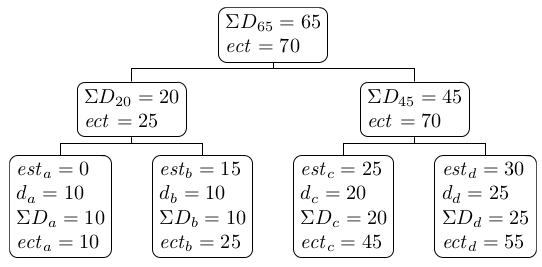
\includegraphics[width=6cm]{img/ecttree.png}
                        \end{center}


                    \item Overload checking : checks that it is possible
                        to schedule all activiites ($\bigoh(n^2)$ or $\bigoh(n log n)$).
                        $$\textrm{Fail if} ect_{\omega} > lct_{\omega}$$
                        \begin{center}
                            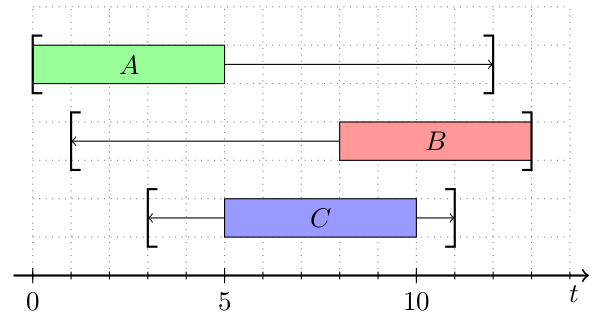
\includegraphics[width=6cm]{img/overload.png}
                        \end{center}


                    \item Detectable precedences : compote the \texttt{ect} of the group
                        to update the \texttt{est} of the activity ($\bigoh(n^2)$ or $\bigoh(n log n)$).
                        $$\forall a_i \in \omega : a_i \prec B (B \notin \omega)
                        \Rightarrow est_i = max( est_B, ect_{\omega})$$
                        \begin{center}
                            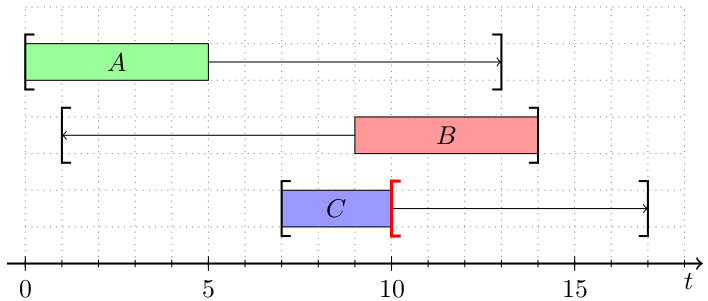
\includegraphics[width=6cm]{img/pred.png}
                        \end{center}

                    \item Not-first/not-last : ($\bigoh(n^2)$ or $\bigoh(n log n)$).
                        $$ect_{\omega} > lst_i \Rightarrow lct_i = min( lct_i, max_{j \in \omega}(lst_j))$$
                        \begin{center}
                            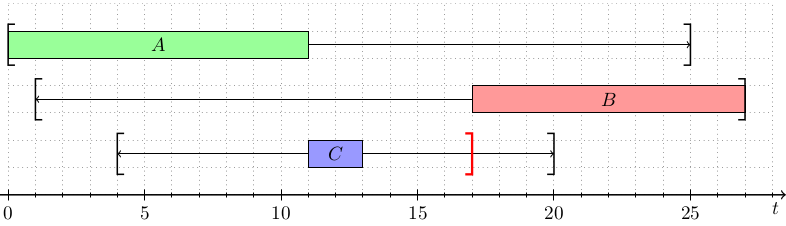
\includegraphics[width=6cm]{img/nfnl.png}
                        \end{center}

                    \item Edge finding : ($\bigoh(n^2)$ or $\bigoh(n log n)$)
                        $$ect_{\omega \cup \{i\}} > lct_{\omega} \Rightarrow \omega \prec i
                        \Rightarrow est_i = max(est_i, ect_{\omega})$$
                        \begin{center}
                            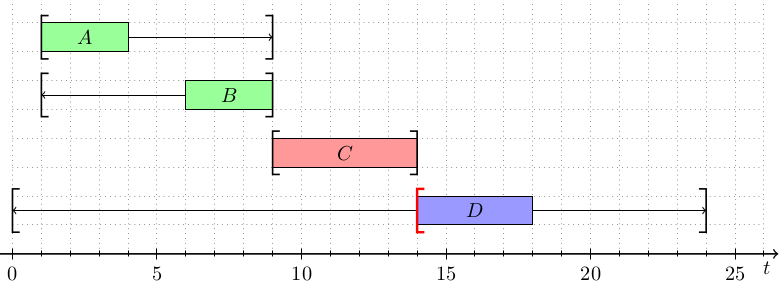
\includegraphics[width=6cm]{img/edge.png}
                        \end{center}

                \end{enumerate}

                \begin{figure}[!h]
                    \centering
                    \begin{tikzpicture}
                        \node[draw, rectangle] (A) {Overload checking};
                        \node[draw, rectangle, below= of A] (B) {Detectable precedences};
                        \node[draw, rectangle, below= of B] (C) {Not-first / Not-last};
                        \node[draw, rectangle, below= of C] (D) {Edge finding};
                        \node[draw, rectangle, below= of D] (E) {Fixpoint};

                        \node[draw, rectangle, right= 2cm of A] (F) {Fail};

                        \path[->] (A) edge node[right] {Consistent} (B)
                        (B) edge node[right] {No change} (C)
                        (C) edge node[right] {No change} (D)
                        (D) edge node[right] {No change} (E)
                        (A) edge node[above] {Fail} (F);

                        \coordinate[below left= of A] (J) ;

                        \draw[->] (B.180) -| (J) |- (A.180);
                        \draw[->] (C.180) -| (J) |- (A.180);
                        \draw[->] (D.180) -| (J) |- (A.180);

                        \node[left=1cm of C] {Change};
                    \end{tikzpicture}
                    \caption{Unary fixpoint}
                \end{figure}


            \item \underline{Cumulative resources} : can be used by activities up to a capacity

                \begin{enumerate}
                    \item Mandatory part
                        \begin{center}
                            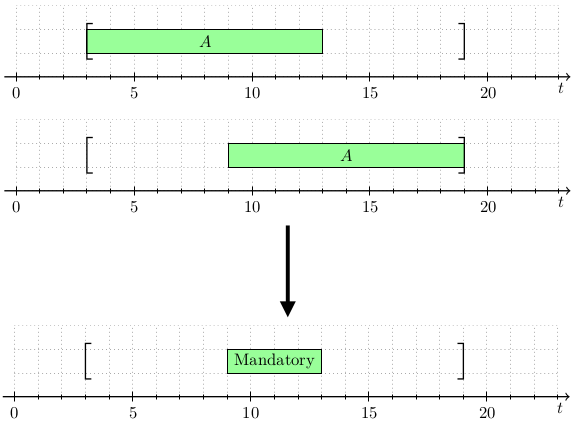
\includegraphics[width=6cm]{img/mandatory.png}
                        \end{center}

                    \item Sweeping algorithm : build resource profile from mandatory parts
                        ($\bigoh(n^2)$ or $\bigoh(n log n)$).

                    \item Energetic reasoning : represent activity comsumption as water
                        and check if all water fits in a bucket ($\bigoh(n^4)$ or $\bigoh(n^3 log n)$)

                \end{enumerate}

            \item \underline{Reservoir resources} : can be consumed or produced by activities
                and usage must remain between lower and upper capacity
        \end{itemize}

        Activities can use a given amount of the resource and modify the state
        of the resource.

    \item A set of \textbf{constraints} $(C = \{c_1,\cdots, c_k\})$

        \begin{itemize}
            \item Resources constraint :
                \begin{tabular}{l}
                    disjunctive resources: not two activities simultaneously\\
                    cumulative resources: cannot exceed capacity\\
                    reservoir resource: quantity between lower/upper capacity\\
                    state resource: resource must be in correct state\\
                \end{tabular}

            \item Time constraints : \begin{tabular}{l}
                    Precedences\\ Max distance between a group of activities \\
                    Transition times
                \end{tabular}

        \end{itemize}

    \item \textbf{Optimization}:
        Minimize: \begin{tabular}{m{2cm}m{4cm}}
            Makespan & 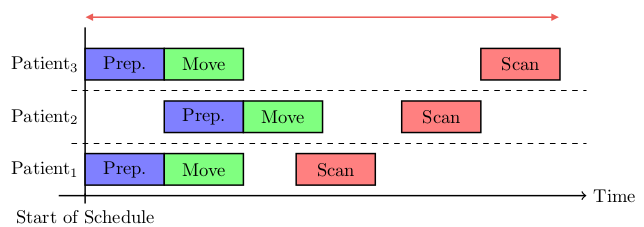
\includegraphics[width=6cm]{img/schedul1.png} \\
            Lateness & 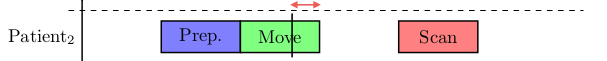
\includegraphics[width=6cm]{img/schedul2.png}\\
            Earliness & 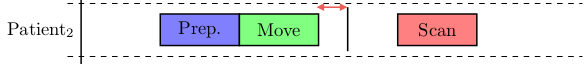
\includegraphics[width=6cm]{img/schedul3.png}\\
            Flast usage of resource & 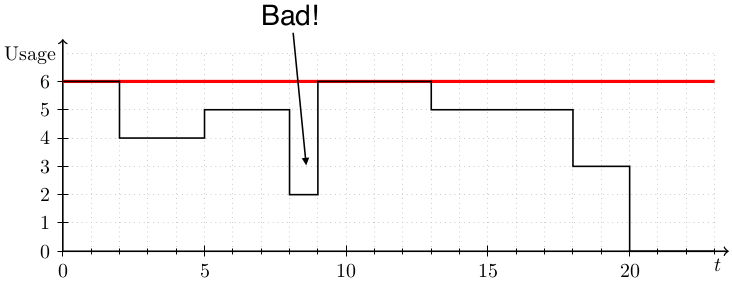
\includegraphics[width=6cm]{img/schedul4.png}\\
        \end{tabular}

\end{itemize}

\subsection{Search}

%TODO

\section{Solver aspect}

\subsection{Restoring state}
\begin{tabular}{m{7cm}m{7cm}}
    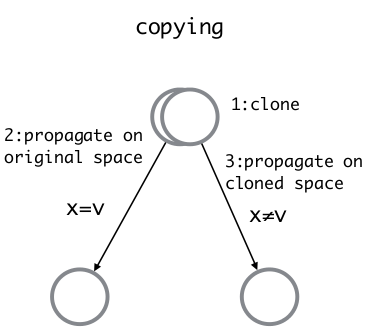
\includegraphics[width=7cm]{img/copying.png}
    &
    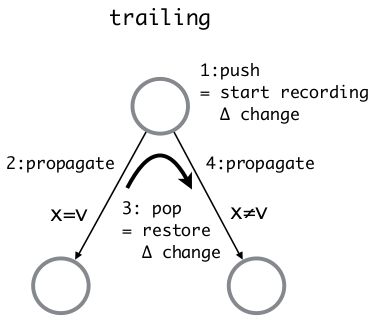
\includegraphics[width=7cm]{img/trailing.png}
    \\
    Easy to make but memory consumption &
    Efficient and increment but difficult to make
\end{tabular}

\subsubsection{Sparse set}
He is us to make a domain representation.

\paragraph{Invariant} :
$ D = \{dom[i] | 0 \leq i \leq size\}$

$map[v] = i \Leftrightarrow dom[i] = v$


\begin{itemize}
    \item Check if v in the domain: $\bigoh(1)$
    \item Remove value c: $\bigoh(1)$
    \item Domain iteration: not possible to iterate increasingly on the value,
        this i a limitation of sparse-sets
\end{itemize}

%TODO

\section{Parallelization}


\section{Examen questions}

\begin{enumerate}
    % 1
    \item \begin{itemize}
            \item Formal definition of CSP
            \item Formal definition of COP
            \item Definition of a constraint
            \item Principle of search in CP
            \item Current DOmain
            \item Communication in CP
            \item Computational model
        \end{itemize}
    % 2
    \item
    % 3
    \item \begin{itemize}
            \item Consistency
            \item Definition of GAC
            \item Value based fixed point
            \item (G)AC3, AC3rm, AC2001, (G)AC4, AC6
            \item Complexities
            \item Invariant on their data structure
        \end{itemize}
    % 4
    \item \begin{itemize}
            \item Fixed point: algorithms, commonalities, differences
            \item Definitions of consistencies : BC, FC, Singleton consitencies,
                Singleton GAC, maxRPWC
            \item Relative strengths of consistencies
            \item Global view on propagation in CP
            \item An algorithm for a consistency inside a fixed point
                for a constraint
            \item How to mix consistencies
        \end{itemize}
    % 5
    \item \begin{itemize}
            \item Depth first backtracking search
            \item How to backtrack information
            \item Branching strategies
            \item First-fail and best-first
            \item Variable ordering heuristics
            \item Values ordering heuristics
            \item Exploration strategies
            \item How to solve constraint optimization problems
        \end{itemize}
    % 6
    \item \begin{itemize}
            \item Example of global constraints
            \item Advantages of global constraints
            \item Decomposition and puning equivalence condition
            \item AllDifferent
            \item Sum constraint
        \end{itemize}
    % 7
    \item \begin{itemize}
            \item GAC propagator for GCC
                \begin{itemize}
                    \item value network
                    \item flow conservation
                    \item redsidual graph
                    \item How to find feasible flow
                    \item How to compute GAC for GCC
                \end{itemize}
            \item TC : STR algorithm, sparse sets for tables
        \end{itemize}

\end{enumerate}

\end{document}
